\section{Results and discussion}\label{sec:results}
The following chapter will present the results of the models presented in Chapter~\ref{sec:methodology} before comparing the different models and discussing the results. We will start by examining the different ARIMA models, from the simplest ARIMA to the more complex SARIMA. We will then compare this to the LSTM model. 

\subsection{ARIMA}\label{sec:arima}
As explained in section \ref{ARIMA and SARIMAX Methodology}, determening the order of the ARIMA model can be a difficult and complex task, examining the ACF and PACF plots can be a good starting point, but will also be a bit subjective. The only objective way to optimize the model is to use a loss function. In our case we have chosen root mean squared error as this is a commonly used way to measure the accuracy of a model.

In order to find the model with the least RMSE, we performed a grid search on the different parameters using a nested for-loop and outputting the results in the following table: 
\begin{table}[H]
    \begin{center}
        \import{data/Figures/ARIMA/}{AutoARIMAResults}
        \caption{Results of the grid search for the ARIMA model.}\label{tab:ARIMAResults}
    \end{center}
\end{table}
Examining table~\ref{tab:ARIMAResults} we can see that the ARIMA(0,1,1) has the lowest RMSE and is therefore expected to be the best model, but there is no significant difference between the models, this may indicate that the model is not able to capture the trends. An ARIMA model with $p$ of 0, $d$ of 1 and $q$ of 1 is, according to \textcite{nau_2019}, a simple exponential smoothing model which indicates that it may capture the moving average trend, but no other trends. Fitting the model to the data and plotting the results against the actual values we get the following plot:
\begin{figure}[H]
    \begin{center}
        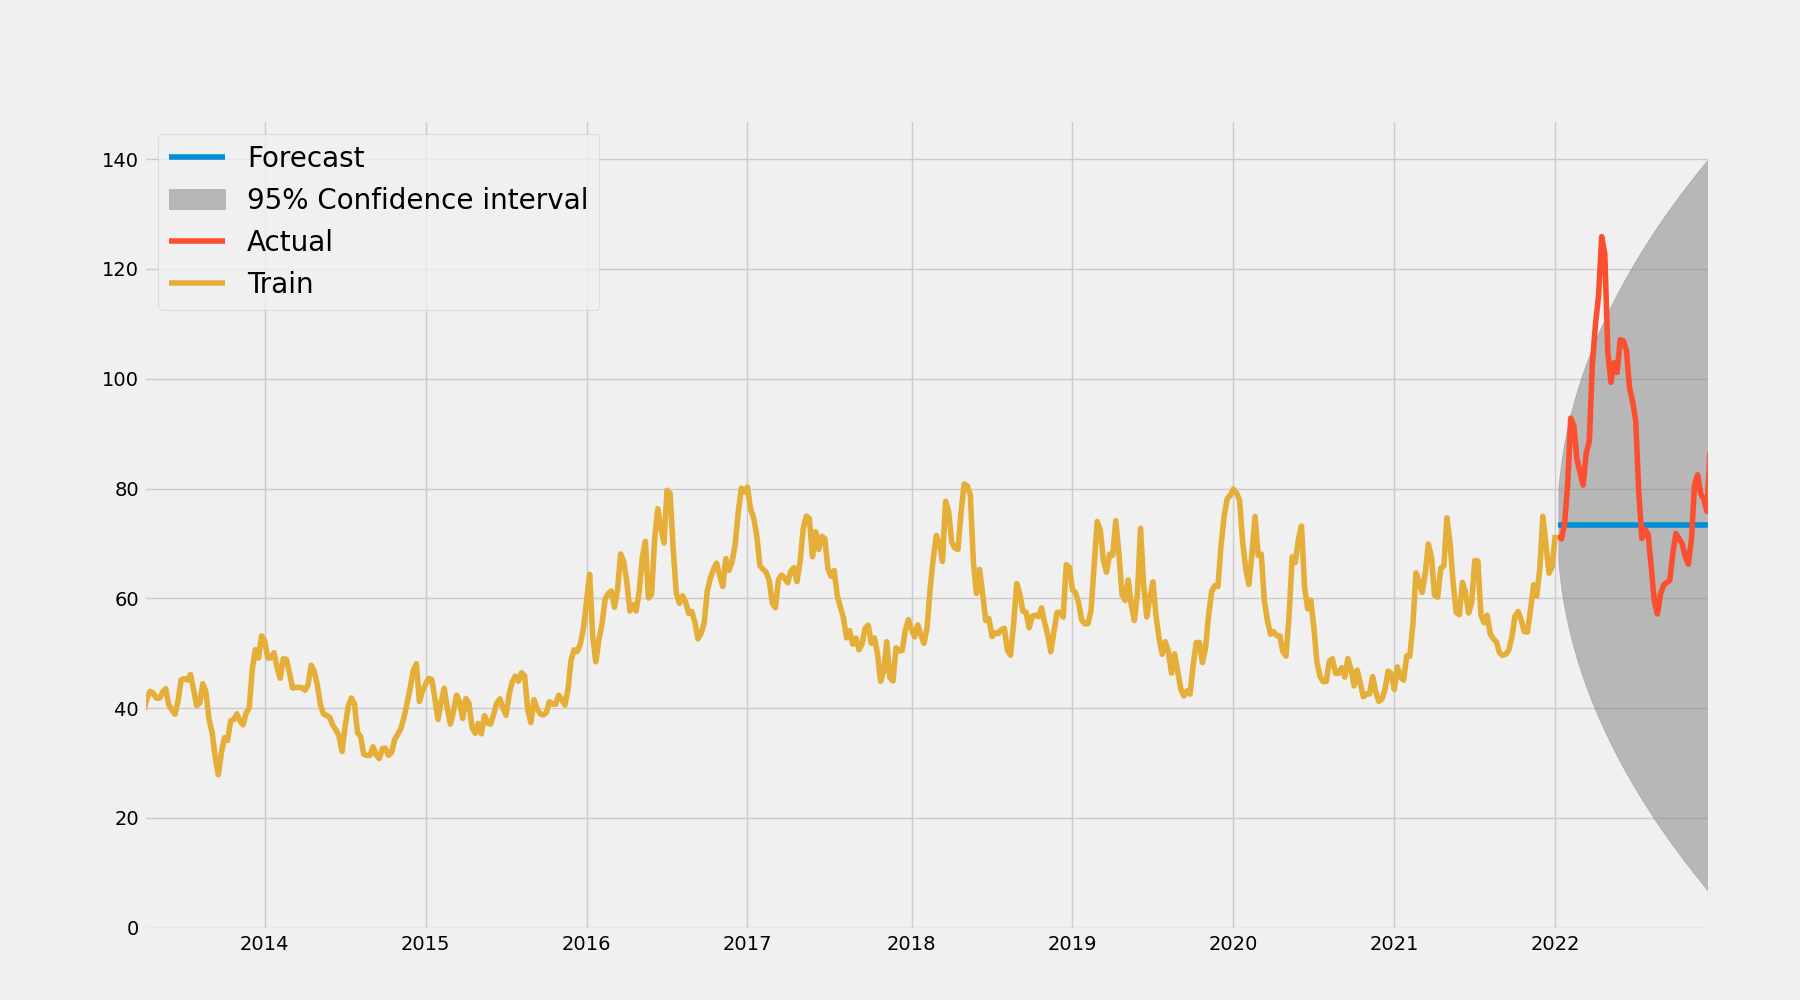
\includegraphics[width=0.9\textwidth]{data/Figures/ARIMA/ARIMA_0_1_1.png}
        \caption{ARIMA(0,1,1) model fitted to the data.}\label{fig:ARIMA_011}
    \end{center}
\end{figure}
As we can see, the model was not able to capture the trend, it seems that it was only able to take the average and draw it further out. In addition, the 95\% confidence interval is very wide, indicating that the model is less than accurate.

Since this was the ARIMA model with the lowest RMSE, there is no reason to believe that the other ARIMA models will be any more accurate. We will therefore not examine the other ARIMA models, but instead move on to the SARIMA models.

\subsection{SARIMA}\label{sec:sarima}
One of the more prominent features of the Salmon data is the clear seasonality that is exhibited on a yearly basis. We should therefore expect a seasonal model to better be able to capture this trend. As we did with the ARIMA models, we will perform a grid search on the different parameters using a nested for-loop, the problem with this is that the SARIMA model has 6 parameters instead of 3. The search will therefore grow exponentially, consequently, we decided to solely use a $P$ of 0, $D$ of 1 and $Q$ of 0 as a larger $P$ and $Q$ seemed to have a negative effect on the RMSE. As the data has a seasonality of 52 weeks, this is the seasonal parameter we will use. The ten best results of the grid search are presented in the following table:
\begin{table}[H]
    \begin{center}
        \import{data/Figures/ARIMA/}{AutoSARIMAResults}
        \caption{Results of the grid search for the SARIMA model.}\label{tab:SARIMAResults}
    \end{center}
\end{table}
Similary to the ARIMA model, there is not a significant difference between the models, but the RMSE is clearly lower in the SARIMA than the ARIMA, this indicates the importance of capturing the seasonal trend in the dataset. The SARIMA(2,1,0)(0,1,0)[52] model has the lowest RMSE and should therefore be the most accurate SARIMA model. After fitting the model on the train data and comparing the predictions against the actual data we get the following plot:
\begin{figure}[H]
    \begin{center}
        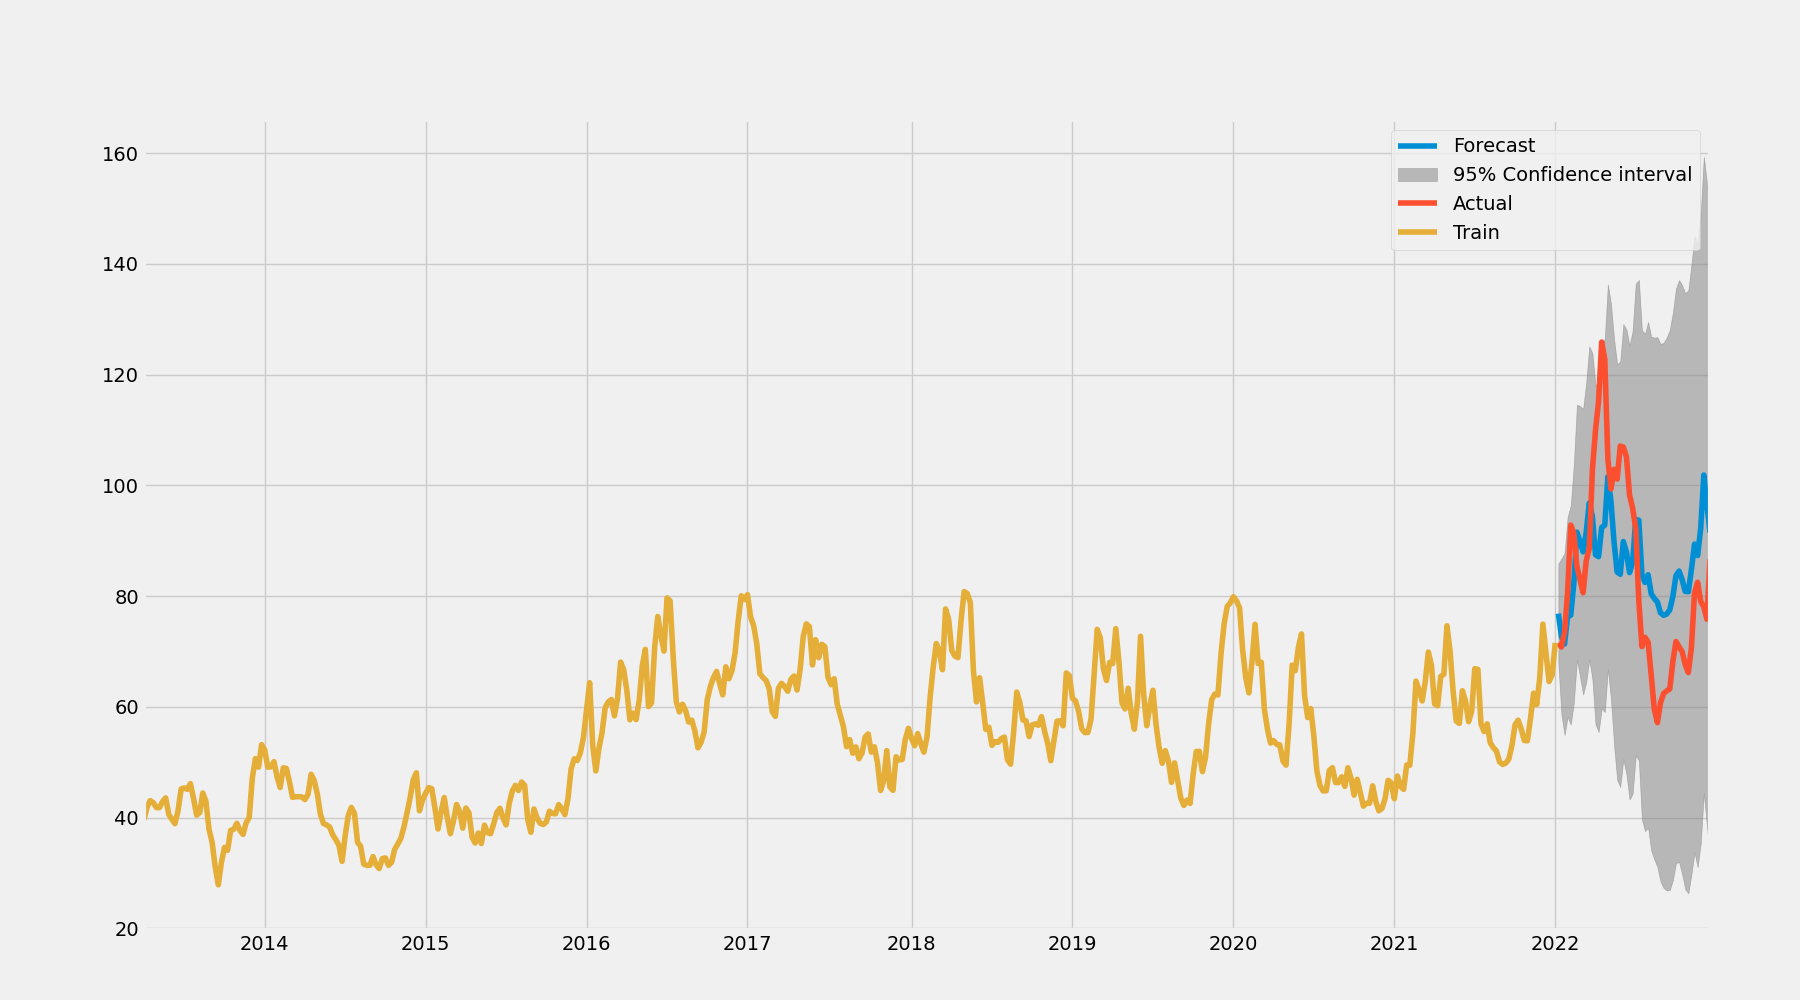
\includegraphics[width=0.9\textwidth]{data/Figures/ARIMA/SARIMA_2_1_0_0_1_0_52.png}
        \caption{SARIMA(2,1,0)(0,1,0)[52] model fitted to the data.}\label{fig:SARIMA_21001052}
    \end{center}
\end{figure}


\subsection{SARIMAX}\label{sec:sarimax}

\subsection{LSTM}\label{sec:lstm}

\subsection{Comparison}\label{sec:comparison}

\subsection{Discussion}\label{sec:discussion}